\chapter{Sistemi di Coordinate e Sistemi di Riferimento}
\label{ch:coordinate_systems}

\section{Introduzione}

La meccanica celeste richiede la specifica precisa di posizioni e velocità. Ciò necessita di \textit{sistemi di coordinate} ben definiti (strutture matematiche per specificare posizioni) e \textit{sistemi di riferimento} (realizzazioni fisiche legate a oggetti astronomici).

\section{Concetti Fondamentali}

\subsection{Sistemi Inerziali vs. Rotanti}

\begin{definition}[Sistema Inerziale]
Un \textit{sistema di riferimento inerziale} è uno in cui vale la prima legge di Newton: un corpo non soggetto a forze si muove in linea retta a velocità costante.
\end{definition}

Sistemi veramente inerziali non esistono (l'universo si espande!), ma sistemi fissi rispetto a quasar distanti sono effettivamente inerziali per la dinamica del sistema solare.

\begin{definition}[Sistema Rotante]
Un \textit{sistema di riferimento rotante} ruota rispetto allo spazio inerziale. Forze fittizie (centrifuga, Coriolis) appaiono nei sistemi rotanti.
\end{definition}

\section{Sistema di Coordinate Equatoriali}

\subsection{Definizione}

Il sistema equatoriale usa l'equatore e l'asse di rotazione terrestre:

\begin{itemize}
    \item \textbf{Piano fondamentale}: Equatore terrestre (esteso alla sfera celeste)
    \item \textbf{Direzione primaria}: Equinozio vernale ($\gamma$), dove il Sole attraversa l'equatore verso nord
    \item \textbf{Polo}: Polo celeste nord (direzione dell'asse di rotazione terrestre)
\end{itemize}

\begin{figure}[H]
\centering
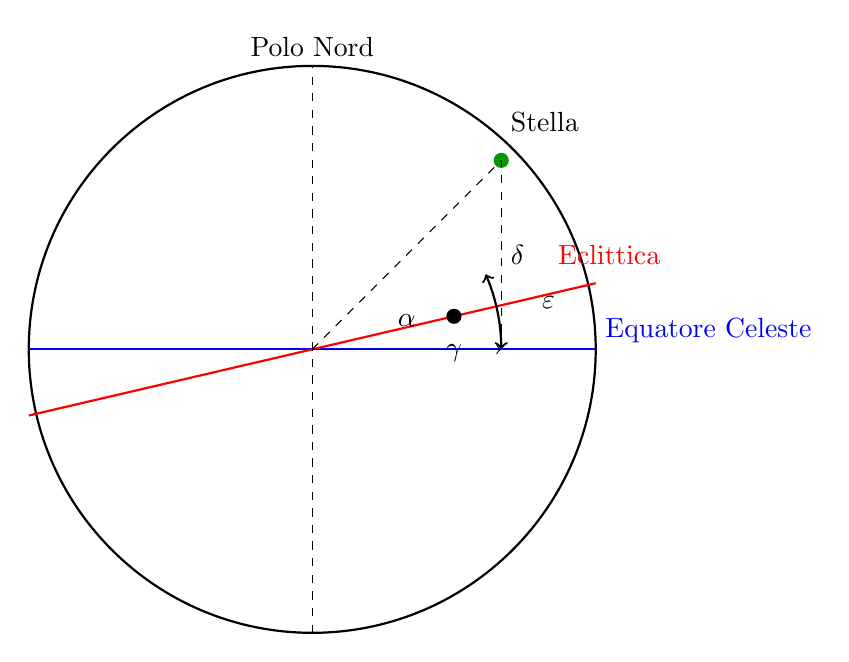
\begin{tikzpicture}[scale=1.2]
    % Celestial sphere
    \draw[thick] (0,0) circle (3);
    
    % Equator
    \draw[thick, blue] (-3,0) -- (3,0);
    \node[blue, right] at (3,0.2) {Equatore Celeste};
    
    % Ecliptic
    \draw[thick, red] (-3,-0.7) -- (3,0.7);
    \node[red, right] at (2.5,1) {Eclittica};
    
    % Vernal equinox
    \fill (1.5,0.35) circle (0.08);
    \node[below] at (1.5,0.15) {$\gamma$};
    
    % Poles
    \draw[dashed] (0,-3) -- (0,3);
    \node[above] at (0,3) {Polo Nord};
    
    % Obliquity
    \draw[<->, thick] (2,0) arc (0:23.4:2);
    \node at (2.5,0.5) {$\varepsilon$};
    
    % Star position
    \fill[green!60!black] (2,2) circle (0.08);
    \draw[dashed] (0,0) -- (2,2);
    \draw[dashed] (2,0) -- (2,2);
    \draw[->] (0,0) -- (2,0);
    \node at (1,0.3) {$\alpha$};
    \node[right] at (2,1) {$\delta$};
    \node[above right] at (2,2.2) {Stella};
\end{tikzpicture}
\caption{Sistema di coordinate equatoriali mostrando ascensione retta ($\alpha$) e declinazione ($\delta$). L'obliquità $\varepsilon \approx 23.4^\circ$.}
\label{fig:equatorial}
\end{figure}

\subsection{Coordinate Sferiche}

Le posizioni sono specificate da:

\begin{description}
    \item[Ascensione Retta ($\alpha$)] Angolo verso est dall'equinozio vernale lungo l'equatore (da $0^\circ$ a $360^\circ$, o da 0h a 24h)
    \item[Declinazione ($\delta$)] Angolo a nord (+) o a sud ($-$) dell'equatore (da $-90^\circ$ a $+90^\circ$)
    \item[Distanza ($r$)] Distanza radiale dall'origine
\end{description}

Conversione in coordinate cartesiane:

\begin{align}
x &= r \cos\delta \cos\alpha \\
y &= r \cos\delta \sin\alpha \\
z &= r \sin\delta
\end{align}

\section{Sistema di Coordinate Eclittiche}

\subsection{Definizione}

Il sistema eclittico usa il piano orbitale terrestre:

\begin{itemize}
    \item \textbf{Piano fondamentale}: Eclittica (piano orbitale terrestre)
    \item \textbf{Direzione primaria}: Equinozio vernale (stesso del sistema equatoriale)
    \item \textbf{Polo}: Normale al piano dell'eclittica
\end{itemize}

Le coordinate sono:
\begin{description}
    \item[Longitudine Eclittica ($\lambda$)] Angolo dall'equinozio vernale lungo l'eclittica
    \item[Latitudine Eclittica ($\beta$)] Angolo a nord/sud dell'eclittica
\end{description}

\subsection{Perché Usare Coordinate Eclittiche?}

Per oggetti del sistema solare:
\begin{itemize}
    \item Le orbite planetarie giacciono vicino all'eclittica ($|\beta| < 10^\circ$ tipicamente)
    \item Semplifica i calcoli di perturbazione
    \item Sistema naturale per la dinamica eliocentrica
\end{itemize}

\section{Trasformazione tra Sistemi}

\subsection{Eclittico $\leftrightarrow$ Equatoriale}

La trasformazione implica una rotazione attorno all'asse $x$ (direzione dell'equinozio vernale) di un angolo pari all'\textit{obliquità} $\varepsilon \approx 23.43929^\circ$:

\begin{equation}
\begin{bmatrix} x \\ y \\ z \end{bmatrix}_{\text{eq}}
= 
\mathbf{R}_x(\varepsilon)
\begin{bmatrix} x \\ y \\ z \end{bmatrix}_{\text{ecl}}
=
\begin{bmatrix}
1 & 0 & 0 \\
0 & \cos\varepsilon & -\sin\varepsilon \\
0 & \sin\varepsilon & \cos\varepsilon
\end{bmatrix}
\begin{bmatrix} x \\ y \\ z \end{bmatrix}_{\text{ecl}}
\end{equation}

Per la trasformazione inversa (equatoriale → eclittico), usare $\mathbf{R}_x(-\varepsilon) = \mathbf{R}_x(\varepsilon)^T$.

\subsection{Implementazione}

\begin{lstlisting}[style=cpp,caption={Trasformazioni di coordinate in AstDyn}]
#include <astdyn/coordinates/ReferenceFrame.hpp>
using namespace astdyn::coordinates;

// Eclittico a equatoriale J2000
Vector3d pos_ecl(1.0, 0.5, 0.1);  // AU
Matrix3d rot = ReferenceFrame::ecliptic_to_j2000();
Vector3d pos_eq = rot * pos_ecl;

// Equatoriale a eclittico
Vector3d vel_eq(0.01, 0.02, 0.005);  // AU/giorno
Matrix3d rot_inv = rot.transpose();  // Matrice ortogonale
Vector3d vel_ecl = rot_inv * vel_eq;
\end{lstlisting}

\section{Il Sistema di Riferimento J2000.0}

\subsection{Epoca vs. Equinozio}

Due concetti temporali sono critici:

\begin{description}
    \item[Epoca] Il tempo per cui sono specificate le coordinate (influenza le posizioni a causa del moto)
    \item[Equinozio] Il tempo che definisce l'orientamento degli assi coordinati (influenza le direzioni di riferimento)
\end{description}

Esempio: "Posizione all'epoca 2025.0 nell'equinozio J2000.0" significa la posizione dell'oggetto al 1 gennaio 2025, espressa in un sistema di coordinate i cui assi sono definiti dall'orientamento terrestre al 1 gennaio 2000.

\subsection{Precessione}

L'asse di rotazione terrestre precede (oscilla) con un periodo di circa 26.000 anni a causa delle forze mareali del Sole e della Luna. Ciò causa la deriva dell'equinozio vernale verso ovest lungo l'eclittica a circa 50'' all'anno.

\begin{figure}[H]
\centering
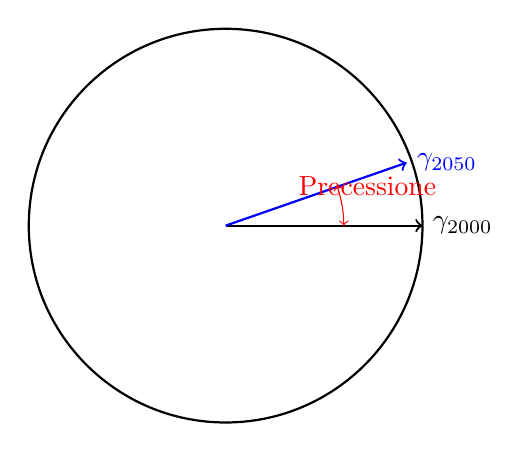
\begin{tikzpicture}
    \draw[thick] (0,0) circle (2.5);
    \draw[thick, ->] (0,0) -- (2.5,0) node[right] {$\gamma_{2000}$};
    \draw[thick, ->, blue] (0,0) -- (2.3,0.8) node[right] {$\gamma_{2050}$};
    \draw[<->, red] (1.5,0) arc (0:20:1.5);
    \node[red] at (1.8,0.5) {Precessione};
\end{tikzpicture}
\caption{Precessione degli equinozi in 50 anni}
\end{figure}

Il sistema J2000.0 fissa l'equinozio al 1 gennaio 2000, 12:00 TT, fornendo un riferimento fisso per calcoli a lungo termine.

\section{Considerazioni Pratiche}

\subsection{Scelta del Sistema di Riferimento}

\begin{itemize}
    \item \textbf{Eclittico eliocentrico}: Naturale per orbite di pianeti/asteroidi
    \item \textbf{Equatoriale geocentrico}: Standard per osservazioni da Terra
    \item \textbf{Baricentrico}: Richiesto per effemeridi planetarie precise
\end{itemize}

\subsection{Trasformazioni di Sistema in AstDyn}

La libreria fornisce matrici di rotazione per trasformazioni comuni:

\begin{lstlisting}[style=cpp,caption={Trasformazioni disponibili}]
// Eclittico <-> Equatoriale (J2000.0)
Matrix3d ecl_to_eq = ReferenceFrame::ecliptic_to_j2000();
Matrix3d eq_to_ecl = ecl_to_eq.transpose();

// ICRS <-> J2000 (piccola correzione di bias)
Matrix3d icrs_to_j2000 = ReferenceFrame::icrs_to_j2000();
\end{lstlisting}

Più trasformazioni (precessione, nutazione, GCRS) sono disponibili per applicazioni avanzate.

\section{Riepilogo}

Punti chiave:
\begin{itemize}
    \item Sistema equatoriale: Legato alla rotazione terrestre (AR, Dec)
    \item Sistema eclittico: Legato all'orbita terrestre (naturale per dinamica eliocentrica)
    \item Trasformazioni: Semplici matrici di rotazione (ortogonali)
    \item J2000.0: Epoca/equinozio standard per l'astrometria moderna
    \item AstDyn: Implementa tutte le trasformazioni comuni in modo efficiente
\end{itemize}